% ------------------------------------------------------------------------------------------------------------------
% Basic configuration and packages
% ------------------------------------------------------------------------------------------------------------------
% Package for discovering wrong and outdated usage of LaTeX.
% More information to be found in l2tabu English version.
\RequirePackage[l2tabu, orthodox]{nag}
% Class of LaTeX document: {size of paper, size of font}[document class]
\documentclass[a4paper,11pt]{article}



% ------------------------------------------------------
% Packages not tied to particular normal language
% ------------------------------------------------------
% This package should improved spaces in the text
\usepackage{microtype}
% Add few important symbols, like text Celcius degree
\usepackage{textcomp}



% ------------------------------------------------------
% Polonization of LaTeX document
% ------------------------------------------------------
% Basic polonization of the text
\usepackage[MeX]{polski}
% Switching on UTF-8 encoding
\usepackage[utf8]{inputenc}
% Adding font Latin Modern
\usepackage{lmodern}
% Package is need for fonts Latin Modern
\usepackage[T1]{fontenc}



% ------------------------------------------------------
% Setting margins
% ------------------------------------------------------
\usepackage[a4paper, total={14cm, 25cm}]{geometry}



% ------------------------------------------------------
% Setting vertical spaces in the text
% ------------------------------------------------------
% Setting space between lines
\renewcommand{\baselinestretch}{1.1}

% Setting space between lines in tables
\renewcommand{\arraystretch}{1.4}



% ------------------------------------------------------
% Packages for scientific papers
% ------------------------------------------------------
% Switching off \lll symbol, that I guess is representing letter "Ł"
% It collide with `amsmath' package's command with the same name
\let\lll\undefined
% Basic package from American Mathematical Society (AMS)
\usepackage[intlimits]{amsmath}
% Equations are numbered separately in every section
\numberwithin{equation}{section}

% Other very useful packages from AMS
\usepackage{amsfonts}
\usepackage{amssymb}
\usepackage{amscd}
\usepackage{amsthm}

% Package with better looking calligraphy fonts
\usepackage{calrsfs}

% Package with better looking greek letters
% Example of use: pi -> \uppi
\usepackage{upgreek}
% Improving look of lambda letter
\let\oldlambda\lambda
\renewcommand{\lambda}{\uplambda}




% ------------------------------------------------------
% BibLaTeX
% ------------------------------------------------------
% Package biblatex, with biber as its backend, allow us to handle
% bibliography entries that use Unicode symbols outside ASCII
% \usepackage[
% language=polish,
% backend=biber,
% style=alphabetic,
% url=false,
% eprint=true,
% ]{biblatex}

% \addbibresource{Logika-i-teoria-mnogości-Bibliography.bib}





% ------------------------------------------------------
% Defining new environments (?)
% ------------------------------------------------------
% Defining enviroment "Wniosek"
% \newtheorem{corollary}{Wniosek}
% \newtheorem{definition}{Definicja}
% \newtheorem{theorem}{Twierdzenie}





% ------------------------------------------------------
% Wonderful package PGF/TikZ
% ------------------------------------------------------
\usepackage{tikz}

\usepackage[dvipsnames,svgnames]{xcolor}

% Loding TikZ libraries

% % Library for positioning nodes
% \usetikzlibrary{positioning}

% % Styles for arrows
% \usepackage{./Local-packages/PGF-TikZ-Arrows-styles}

% % Node and pics for drawing charts
% \usepackage{./Local-packages/PGF-TikZ-Chart-nodes-and-pics}




% ------------------------------------------------------
% Local packages
% ------------------------------------------------------
% Local configuration of this particular file
\usepackage{./Local-packages/local-settings}

% Package containing various command useful for working with a text
% \usepackage{general-commands}
% Package containing commands and other code useful for working with
% mathematical text
% \usepackage{math-commands}





% ------------------------------------------------------
% Package "hyperref"
% They advised to put it on the end of preambule
% ------------------------------------------------------
% It allows you to use hyperlinks in the text
\usepackage{hyperref}










% ------------------------------------------------------------------------------------------------------------------
% Title and author of the text
\title{Kolory z~paczki \texttt{xcolor}}

\author{Kamil Ziemian \\
  \email}


% \date{}
% ------------------------------------------------------------------------------------------------------------------










% ####################################################################
% Beginning of the document
\begin{document}
% ####################################################################





% ######################################
% Title of the text
\maketitle
% ######################################





% % ######################################
% \section{Gładkie funkcje o~zwartym nośniku}

% \label{sec:Funkcje-wykladnicze-i-logarytmiczne}
% % ######################################



% ##################
\begin{figure}

  \centering


  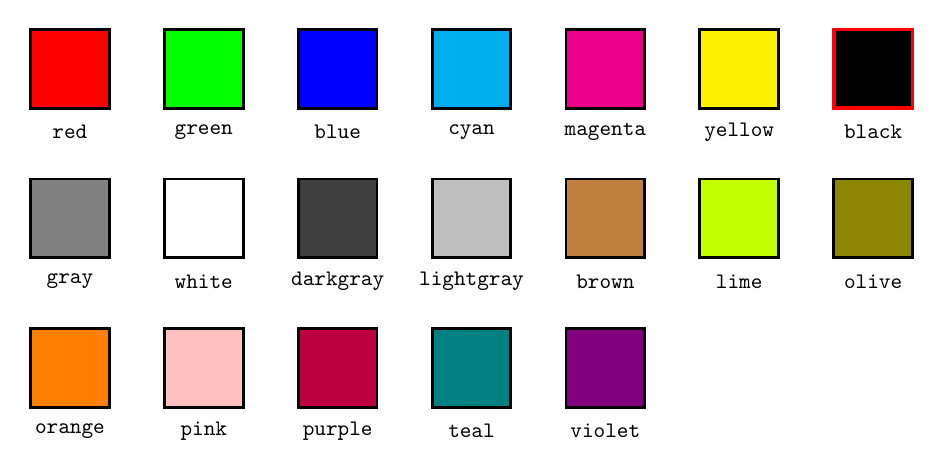
\begin{tikzpicture}

    \filldraw[draw=black,line width=1,fill=red] (0,0) rectangle (1,1);

    \node[scale=0.8] at (0.5,-0.3) {\texttt{red}};



    \begin{scope}[xshift=1.7cm]

      \filldraw[draw=black,line width=1,fill=green] (0,0) rectangle (1,1);

      \node[scale=0.8] at (0.5,-0.3) {\texttt{green}};

    \end{scope}



    \begin{scope}[xshift=3.4cm]

      \filldraw[draw=black,line width=1,fill=blue] (0,0) rectangle (1,1);

      \node[scale=0.8] at (0.5,-0.3) {\texttt{blue}};

    \end{scope}



    \begin{scope}[xshift=5.1cm]

      \filldraw[draw=black,line width=1,fill=cyan] (0,0) rectangle (1,1);

      \node[scale=0.8] at (0.5,-0.3) {\texttt{cyan}};

    \end{scope}



    \begin{scope}[xshift=6.8cm]

      \filldraw[draw=black,line width=1,fill=magenta] (0,0) rectangle (1,1);

      \node[scale=0.8] at (0.5,-0.3) {\texttt{magenta}};

    \end{scope}



    \begin{scope}[xshift=8.5cm]

      \filldraw[draw=black,line width=1,fill=yellow] (0,0) rectangle (1,1);

      \node[scale=0.8] at (0.5,-0.3) {\texttt{yellow}};

    \end{scope}



    \begin{scope}[xshift=10.2cm]

      \filldraw[draw=red,line width=1.3,fill=black] (0,0) rectangle (1,1);

      \node[scale=0.8] at (0.5,-0.3) {\texttt{black}};

    \end{scope}





    \begin{scope}[yshift=-1.9cm]

      \filldraw[draw=black,line width=1,fill=gray] (0,0) rectangle (1,1);

      \node[scale=0.8] at (0.5,-0.3) {\texttt{gray}};

    \end{scope}



    \begin{scope}[xshift=1.7cm,yshift=-1.9cm]

      \filldraw[draw=black,line width=1,fill=white] (0,0) rectangle (1,1);

      \node[scale=0.8] at (0.5,-0.3) {\texttt{white}};

    \end{scope}



    \begin{scope}[xshift=3.4cm,yshift=-1.9cm]

      \filldraw[draw=black,line width=1,fill=darkgray]
      (0,0) rectangle (1,1);

      \node[scale=0.8] at (0.5,-0.3) {\texttt{darkgray}};

    \end{scope}



    \begin{scope}[xshift=5.1cm,yshift=-1.9cm]

      \filldraw[draw=black,line width=1,fill=lightgray]
      (0,0) rectangle (1,1);

      \node[scale=0.8] at (0.5,-0.3) {\texttt{lightgray}};

    \end{scope}



    \begin{scope}[xshift=6.8cm,yshift=-1.9cm]

      \filldraw[draw=black,line width=1,fill=brown] (0,0) rectangle (1,1);

      \node[scale=0.8] at (0.5,-0.3) {\texttt{brown}};

    \end{scope}



    \begin{scope}[xshift=8.5cm,yshift=-1.9cm]

      \filldraw[draw=black,line width=1,fill=lime] (0,0) rectangle (1,1);

      \node[scale=0.8] at (0.5,-0.3) {\texttt{lime}};

    \end{scope}



    \begin{scope}[xshift=10.2cm,yshift=-1.9cm]

      \filldraw[draw=black,line width=1,fill=olive] (0,0) rectangle (1,1);

      \node[scale=0.8] at (0.5,-0.3) {\texttt{olive}};

    \end{scope}





    \begin{scope}[yshift=-3.8cm]

      \filldraw[draw=black,line width=1,fill=orange] (0,0) rectangle (1,1);

      \node[scale=0.8] at (0.5,-0.3) {\texttt{orange}};

    \end{scope}



    \begin{scope}[xshift=1.7cm,yshift=-3.8cm]

      \filldraw[draw=black,line width=1,fill=pink] (0,0) rectangle (1,1);

      \node[scale=0.8] at (0.5,-0.3) {\texttt{pink}};

    \end{scope}



    \begin{scope}[xshift=3.4cm,yshift=-3.8cm]

      \filldraw[draw=black,line width=1,fill=purple] (0,0) rectangle (1,1);

      \node[scale=0.8] at (0.5,-0.3) {\texttt{purple}};

    \end{scope}



    \begin{scope}[xshift=5.1cm,yshift=-3.8cm]

      \filldraw[draw=black,line width=1,fill=teal] (0,0) rectangle (1,1);

      \node[scale=0.8] at (0.5,-0.3) {\texttt{teal}};

    \end{scope}



    \begin{scope}[xshift=6.8cm,yshift=-3.8cm]

      \filldraw[draw=black,line width=1,fill=violet]
      (0,0) rectangle (1,1);

      \node[scale=0.8] at (0.5,-0.3) {\texttt{violet}};

    \end{scope}

  \end{tikzpicture}

  \caption{Kolor bazowe paczki
    \href{https://ctan.org/pkg/xcolor}{\texttt{xcolor}}}


  \label{fig:Basic-colors}

\end{figure}
% ##################





% ##################
\begin{figure}

  \centering


  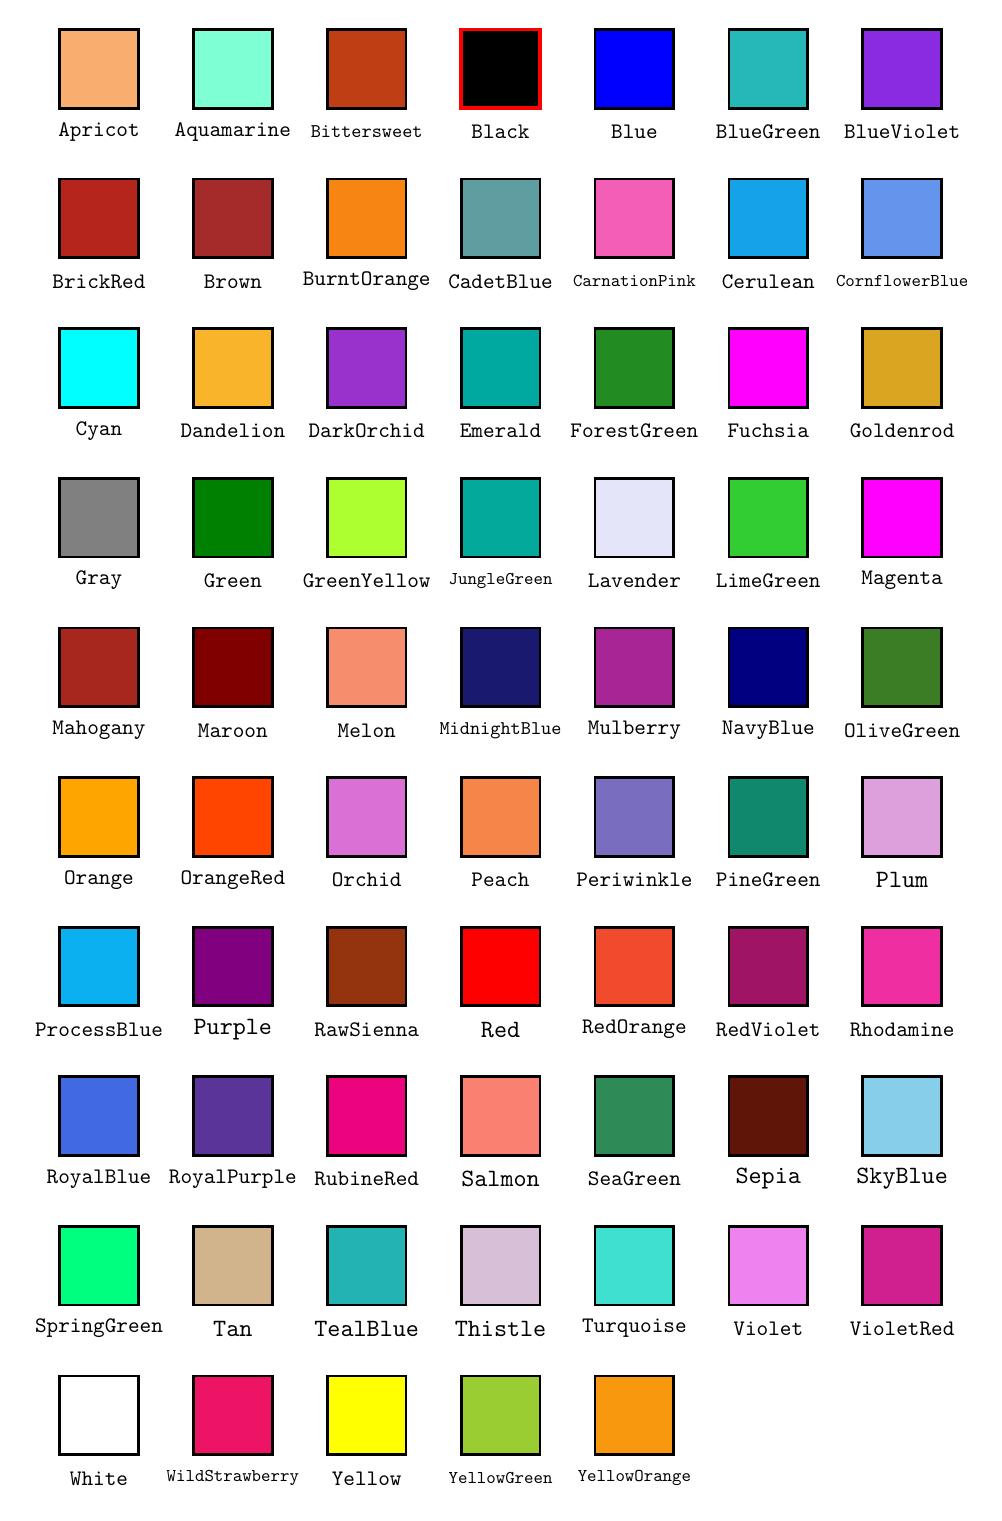
\begin{tikzpicture}

    \filldraw[draw=black,line width=1,fill=Apricot] (0,0) rectangle (1,1);

    \node[scale=0.8] at (0.5,-0.3) {\texttt{Apricot}};



    \begin{scope}[xshift=1.7cm]

      \filldraw[draw=black,line width=1,fill=Aquamarine]
      (0,0) rectangle (1,1);

      \node[scale=0.8] at (0.5,-0.3) {\texttt{Aquamarine}};

    \end{scope}



    \begin{scope}[xshift=3.4cm]

      \filldraw[draw=black,line width=1,fill=Bittersweet]
      (0,0) rectangle (1,1);

      \node[scale=0.7] at (0.5,-0.3) {\texttt{Bittersweet}};

    \end{scope}



    \begin{scope}[xshift=5.1cm]

      \filldraw[draw=red,line width=1.3,fill=Black] (0,0) rectangle (1,1);

      \node[scale=0.8] at (0.5,-0.3) {\texttt{Black}};

    \end{scope}



    \begin{scope}[xshift=6.8cm]

      \filldraw[draw=black,line width=1,fill=Blue] (0,0) rectangle (1,1);

      \node[scale=0.8] at (0.5,-0.3) {\texttt{Blue}};

    \end{scope}



    \begin{scope}[xshift=8.5cm]

      \filldraw[draw=black,line width=1,fill=BlueGreen]
      (0,0) rectangle (1,1);

      \node[scale=0.8] at (0.5,-0.3) {\texttt{BlueGreen}};

    \end{scope}



    \begin{scope}[xshift=10.2cm]

      \filldraw[draw=black,line width=1,fill=BlueViolet]
      (0,0) rectangle (1,1);

      \node[scale=0.8] at (0.5,-0.3) {\texttt{BlueViolet}};

    \end{scope}





    \begin{scope}[yshift=-1.9cm]

      \filldraw[draw=black,line width=1,fill=BrickRed]
      (0,0) rectangle (1,1);

      \node[scale=0.8] at (0.5,-0.3) {\texttt{BrickRed}};

    \end{scope}



    \begin{scope}[xshift=1.7cm,yshift=-1.9cm]

      \filldraw[draw=black,line width=1,fill=Brown] (0,0) rectangle (1,1);

      \node[scale=0.8] at (0.5,-0.3) {\texttt{Brown}};

    \end{scope}



    \begin{scope}[xshift=3.4cm,yshift=-1.9cm]

      \filldraw[draw=black,line width=1,fill=BurntOrange]
      (0,0) rectangle (1,1);

      \node[scale=0.8] at (0.5,-0.3) {\texttt{BurntOrange}};

    \end{scope}



    \begin{scope}[xshift=5.1cm,yshift=-1.9cm]

      \filldraw[draw=black,line width=1,fill=CadetBlue]
      (0,0) rectangle (1,1);

      \node[scale=0.8] at (0.5,-0.3) {\texttt{CadetBlue}};

    \end{scope}



    \begin{scope}[xshift=6.8cm,yshift=-1.9cm]

      \filldraw[draw=black,line width=1,fill=CarnationPink]
      (0,0) rectangle (1,1);

      \node[scale=0.65] at (0.5,-0.3) {\texttt{CarnationPink}};

    \end{scope}



    \begin{scope}[xshift=8.5cm,yshift=-1.9cm]

      \filldraw[draw=black,line width=1,fill=Cerulean]
      (0,0) rectangle (1,1);

      \node[scale=0.8] at (0.5,-0.3) {\texttt{Cerulean}};

    \end{scope}



    \begin{scope}[xshift=10.2cm,yshift=-1.9cm]

      \filldraw[draw=black,line width=1,fill=CornflowerBlue]
      (0,0) rectangle (1,1);

      \node[scale=0.65] at (0.5,-0.3) {\texttt{CornflowerBlue}};

    \end{scope}





    \begin{scope}[yshift=-3.8cm]

      \filldraw[draw=black,line width=1,fill=Cyan] (0,0) rectangle (1,1);

      \node[scale=0.8] at (0.5,-0.3) {\texttt{Cyan}};

    \end{scope}



    \begin{scope}[xshift=1.7cm,yshift=-3.8cm]

      \filldraw[draw=black,line width=1,fill=Dandelion]
      (0,0) rectangle (1,1);

      \node[scale=0.8] at (0.5,-0.3) {\texttt{Dandelion}};

    \end{scope}



    \begin{scope}[xshift=3.4cm,yshift=-3.8cm]

      \filldraw[draw=black,line width=1,fill=DarkOrchid]
      (0,0) rectangle (1,1);

      \node[scale=0.8] at (0.5,-0.3) {\texttt{DarkOrchid}};

    \end{scope}



    \begin{scope}[xshift=5.1cm,yshift=-3.8cm]

      \filldraw[draw=black,line width=1,fill=Emerald]
      (0,0) rectangle (1,1);

      \node[scale=0.8] at (0.5,-0.3) {\texttt{Emerald}};

    \end{scope}



    \begin{scope}[xshift=6.8cm,yshift=-3.8cm]

      \filldraw[draw=black,line width=1,fill=ForestGreen]
      (0,0) rectangle (1,1);

      \node[scale=0.8] at (0.5,-0.3) {\texttt{ForestGreen}};

    \end{scope}



    \begin{scope}[xshift=8.5cm,yshift=-3.8cm]

      \filldraw[draw=black,line width=1,fill=Fuchsia]
      (0,0) rectangle (1,1);

      \node[scale=0.8] at (0.5,-0.3) {\texttt{Fuchsia}};

    \end{scope}



    \begin{scope}[xshift=10.2cm,yshift=-3.8cm]

      \filldraw[draw=black,line width=1,fill=Goldenrod]
      (0,0) rectangle (1,1);

      \node[scale=0.8] at (0.5,-0.3) {\texttt{Goldenrod}};

    \end{scope}





    \begin{scope}[yshift=-5.7cm]

      \filldraw[draw=black,line width=1,fill=Gray] (0,0) rectangle (1,1);

      \node[scale=0.8] at (0.5,-0.3) {\texttt{Gray}};

    \end{scope}



    \begin{scope}[xshift=1.7cm,yshift=-5.7cm]

      \filldraw[draw=black,line width=1,fill=Green] (0,0) rectangle (1,1);

      \node[scale=0.8] at (0.5,-0.3) {\texttt{Green}};

    \end{scope}



    \begin{scope}[xshift=3.4cm,yshift=-5.7cm]

      \filldraw[draw=black,line width=1,fill=GreenYellow]
      (0,0) rectangle (1,1);

      \node[scale=0.8] at (0.5,-0.3) {\texttt{GreenYellow}};

    \end{scope}



    \begin{scope}[xshift=5.1cm,yshift=-5.7cm]

      \filldraw[draw=black,line width=1,fill=JungleGreen]
      (0,0) rectangle (1,1);

      \node[scale=0.65] at (0.5,-0.3) {\texttt{JungleGreen}};

    \end{scope}



    \begin{scope}[xshift=6.8cm,yshift=-5.7cm]

      \filldraw[draw=black,line width=1,fill=Lavender]
      (0,0) rectangle (1,1);

      \node[scale=0.8] at (0.5,-0.3) {\texttt{Lavender}};

    \end{scope}



    \begin{scope}[xshift=8.5cm,yshift=-5.7cm]

      \filldraw[draw=black,line width=1,fill=LimeGreen]
      (0,0) rectangle (1,1);

      \node[scale=0.8] at (0.5,-0.3) {\texttt{LimeGreen}};

    \end{scope}



    \begin{scope}[xshift=10.2cm,yshift=-5.7cm]

      \filldraw[draw=black,line width=1,fill=Magenta] (0,0) rectangle (1,1);

      \node[scale=0.8] at (0.5,-0.3) {\texttt{Magenta}};

    \end{scope}





    \begin{scope}[yshift=-7.6cm]

      \filldraw[draw=black,line width=1,fill=Mahogany]
      (0,0) rectangle (1,1);

      \node[scale=0.8] at (0.5,-0.3) {\texttt{Mahogany}};

    \end{scope}



    \begin{scope}[xshift=1.7cm,yshift=-7.6cm]

      \filldraw[draw=black,line width=1,fill=Maroon] (0,0) rectangle (1,1);

      \node[scale=0.8] at (0.5,-0.3) {\texttt{Maroon}};

    \end{scope}



    \begin{scope}[xshift=3.4cm,yshift=-7.6cm]

      \filldraw[draw=black,line width=1,fill=Melon] (0,0) rectangle (1,1);

      \node[scale=0.8] at (0.5,-0.3) {\texttt{Melon}};

    \end{scope}



    \begin{scope}[xshift=5.1cm,yshift=-7.6cm]

      \filldraw[draw=black,line width=1,fill=MidnightBlue]
      (0,0) rectangle (1,1);

      \node[scale=0.7] at (0.5,-0.3) {\texttt{MidnightBlue}};

    \end{scope}



    \begin{scope}[xshift=6.8cm,yshift=-7.6cm]

      \filldraw[draw=black,line width=1,fill=Mulberry]
      (0,0) rectangle (1,1);

      \node[scale=0.8] at (0.5,-0.3) {\texttt{Mulberry}};

    \end{scope}



    \begin{scope}[xshift=8.5cm,yshift=-7.6cm]

      \filldraw[draw=black,line width=1,fill=NavyBlue]
      (0,0) rectangle (1,1);

      \node[scale=0.8] at (0.5,-0.3) {\texttt{NavyBlue}};

    \end{scope}



    \begin{scope}[xshift=10.2cm,yshift=-7.6cm]

      \filldraw[draw=black,line width=1,fill=OliveGreen]
      (0,0) rectangle (1,1);

      \node[scale=0.8] at (0.5,-0.3) {\texttt{OliveGreen}};

    \end{scope}





    \begin{scope}[yshift=-9.5cm]

      \filldraw[draw=black,line width=1,fill=Orange] (0,0) rectangle (1,1);

      \node[scale=0.8] at (0.5,-0.3) {\texttt{Orange}};

    \end{scope}



    \begin{scope}[xshift=1.7cm,yshift=-9.5cm]

      \filldraw[draw=black,line width=1,fill=OrangeRed]
      (0,0) rectangle (1,1);

      \node[scale=0.8] at (0.5,-0.3) {\texttt{OrangeRed}};

    \end{scope}



    \begin{scope}[xshift=3.4cm,yshift=-9.5cm]

      \filldraw[draw=black,line width=1,fill=Orchid] (0,0) rectangle (1,1);

      \node[scale=0.8] at (0.5,-0.3) {\texttt{Orchid}};

    \end{scope}



    \begin{scope}[xshift=5.1cm,yshift=-9.5cm]

      \filldraw[draw=black,line width=1,fill=Peach] (0,0) rectangle (1,1);

      \node[scale=0.8] at (0.5,-0.3) {\texttt{Peach}};

    \end{scope}



    \begin{scope}[xshift=6.8cm,yshift=-9.5cm]

      \filldraw[draw=black,line width=1,fill=Periwinkle]
      (0,0) rectangle (1,1);

      \node[scale=0.8] at (0.5,-0.3) {\texttt{Periwinkle}};

    \end{scope}



    \begin{scope}[xshift=8.5cm,yshift=-9.5cm]

      \filldraw[draw=black,line width=1,fill=PineGreen]
      (0,0) rectangle (1,1);

      \node[scale=0.8] at (0.5,-0.3) {\texttt{PineGreen}};

    \end{scope}



    \begin{scope}[xshift=10.2cm,yshift=-9.5cm]

      \filldraw[draw=black,line width=1,fill=Plum] (0,0) rectangle (1,1);

      \node[scale=0.9] at (0.5,-0.3) {\texttt{Plum}};

    \end{scope}





    \begin{scope}[yshift=-11.4cm]

      \filldraw[draw=black,line width=1,fill=ProcessBlue]
      (0,0) rectangle (1,1);

      \node[scale=0.8] at (0.5,-0.3) {\texttt{ProcessBlue}};

    \end{scope}



    \begin{scope}[xshift=1.7cm,yshift=-11.4cm]

      \filldraw[draw=black,line width=1,fill=Purple] (0,0) rectangle (1,1);

      \node[scale=0.9] at (0.5,-0.3) {\texttt{Purple}};

    \end{scope}



    \begin{scope}[xshift=3.4cm,yshift=-11.4cm]

      \filldraw[draw=black,line width=1,fill=RawSienna]
      (0,0) rectangle (1,1);

      \node[scale=0.8] at (0.5,-0.3) {\texttt{RawSienna}};

    \end{scope}



    \begin{scope}[xshift=5.1cm,yshift=-11.4cm]

      \filldraw[draw=black,line width=1,fill=Red] (0,0) rectangle (1,1);

      \node[scale=0.9] at (0.5,-0.3) {\texttt{Red}};

    \end{scope}



    \begin{scope}[xshift=6.8cm,yshift=-11.4cm]

      \filldraw[draw=black,line width=1,fill=RedOrange]
      (0,0) rectangle (1,1);

      \node[scale=0.8] at (0.5,-0.3) {\texttt{RedOrange}};

    \end{scope}



    \begin{scope}[xshift=8.5cm,yshift=-11.4cm]

      \filldraw[draw=black,line width=1,fill=RedViolet]
      (0,0) rectangle (1,1);

      \node[scale=0.8] at (0.5,-0.3) {\texttt{RedViolet}};

    \end{scope}



    \begin{scope}[xshift=10.2cm,yshift=-11.4cm]

      \filldraw[draw=black,line width=1,fill=Rhodamine]
      (0,0) rectangle (1,1);

      \node[scale=0.8] at (0.5,-0.3) {\texttt{Rhodamine}};

    \end{scope}





    \begin{scope}[yshift=-13.3cm]

      \filldraw[draw=black,line width=1,fill=RoyalBlue]
      (0,0) rectangle (1,1);

      \node[scale=0.8] at (0.5,-0.3) {\texttt{RoyalBlue}};

    \end{scope}



    \begin{scope}[xshift=1.7cm,yshift=-13.3cm]

      \filldraw[draw=black,line width=1,fill=RoyalPurple]
      (0,0) rectangle (1,1);

      \node[scale=0.8] at (0.5,-0.3) {\texttt{RoyalPurple}};

    \end{scope}



    \begin{scope}[xshift=3.4cm,yshift=-13.3cm]

      \filldraw[draw=black,line width=1,fill=RubineRed]
      (0,0) rectangle (1,1);

      \node[scale=0.8] at (0.5,-0.3) {\texttt{RubineRed}};

    \end{scope}



    \begin{scope}[xshift=5.1cm,yshift=-13.3cm]

      \filldraw[draw=black,line width=1,fill=Salmon]
      (0,0) rectangle (1,1);

      \node[scale=0.9] at (0.5,-0.3) {\texttt{Salmon}};

    \end{scope}



    \begin{scope}[xshift=6.8cm,yshift=-13.3cm]

      \filldraw[draw=black,line width=1,fill=SeaGreen]
      (0,0) rectangle (1,1);

      \node[scale=0.8] at (0.5,-0.3) {\texttt{SeaGreen}};

    \end{scope}



    \begin{scope}[xshift=8.5cm,yshift=-13.3cm]

      \filldraw[draw=black,line width=1,fill=Sepia] (0,0) rectangle (1,1);

      \node[scale=0.9] at (0.5,-0.3) {\texttt{Sepia}};

    \end{scope}



    \begin{scope}[xshift=10.2cm,yshift=-13.3cm]

      \filldraw[draw=black,line width=1,fill=SkyBlue] (0,0) rectangle (1,1);

      \node[scale=0.9] at (0.5,-0.3) {\texttt{SkyBlue}};

    \end{scope}





    \begin{scope}[yshift=-15.2cm]

      \filldraw[draw=black,line width=1,fill=SpringGreen]
      (0,0) rectangle (1,1);

      \node[scale=0.8] at (0.5,-0.3) {\texttt{SpringGreen}};

    \end{scope}



    \begin{scope}[xshift=1.7cm,yshift=-15.2cm]

      \filldraw[draw=black,line width=1,fill=Tan] (0,0) rectangle (1,1);

      \node[scale=0.9] at (0.5,-0.3) {\texttt{Tan}};

    \end{scope}



    \begin{scope}[xshift=3.4cm,yshift=-15.2cm]

      \filldraw[draw=black,line width=1,fill=TealBlue]
      (0,0) rectangle (1,1);

      \node[scale=0.9] at (0.5,-0.3) {\texttt{TealBlue}};

    \end{scope}



    \begin{scope}[xshift=5.1cm,yshift=-15.2cm]

      \filldraw[draw=black,line width=1,fill=Thistle] (0,0) rectangle (1,1);

      \node[scale=0.9] at (0.5,-0.3) {\texttt{Thistle}};

    \end{scope}



    \begin{scope}[xshift=6.8cm,yshift=-15.2cm]

      \filldraw[draw=black,line width=1,fill=Turquoise]
      (0,0) rectangle (1,1);

      \node[scale=0.8] at (0.5,-0.3) {\texttt{Turquoise}};

    \end{scope}



    \begin{scope}[xshift=8.5cm,yshift=-15.2cm]

      \filldraw[draw=black,line width=1,fill=Violet] (0,0) rectangle (1,1);

      \node[scale=0.8] at (0.5,-0.3) {\texttt{Violet}};

    \end{scope}



    \begin{scope}[xshift=10.2cm,yshift=-15.2cm]

      \filldraw[draw=black,line width=1,fill=VioletRed]
      (0,0) rectangle (1,1);

      \node[scale=0.8] at (0.5,-0.3) {\texttt{VioletRed}};

    \end{scope}





    \begin{scope}[yshift=-17.1cm]

      \filldraw[draw=black,line width=1,fill=White]
      (0,0) rectangle (1,1);

      \node[scale=0.8] at (0.5,-0.3) {\texttt{White}};

    \end{scope}



    \begin{scope}[xshift=1.7cm,yshift=-17.1cm]

      \filldraw[draw=black,line width=1,fill=WildStrawberry]
      (0,0) rectangle (1,1);

      \node[scale=0.65] at (0.5,-0.3) {\texttt{WildStrawberry}};

    \end{scope}



    \begin{scope}[xshift=3.4cm,yshift=-17.1cm]

      \filldraw[draw=black,line width=1,fill=Yellow] (0,0) rectangle (1,1);

      \node[scale=0.8] at (0.5,-0.3) {\texttt{Yellow}};

    \end{scope}



    \begin{scope}[xshift=5.1cm,yshift=-17.1cm]

      \filldraw[draw=black,line width=1,fill=YellowGreen]
      (0,0) rectangle (1,1);

      \node[scale=0.65] at (0.5,-0.3) {\texttt{YellowGreen}};

    \end{scope}



    \begin{scope}[xshift=6.8cm,yshift=-17.1cm]

      \filldraw[draw=black,line width=1,fill=YellowOrange]
      (0,0) rectangle (1,1);

      \node[scale=0.65] at (0.5,-0.3) {\texttt{YellowOrange}};

    \end{scope}

  \end{tikzpicture}

  \caption{Kolor grupy \texttt{dvipsnames} z~paczki
    \href{https://ctan.org/pkg/xcolor}{\texttt{xcolor}}}


  \label{fig:dvipsnames-colors}

\end{figure}
% ##################





% ##################
\begin{figure}

  \centering


  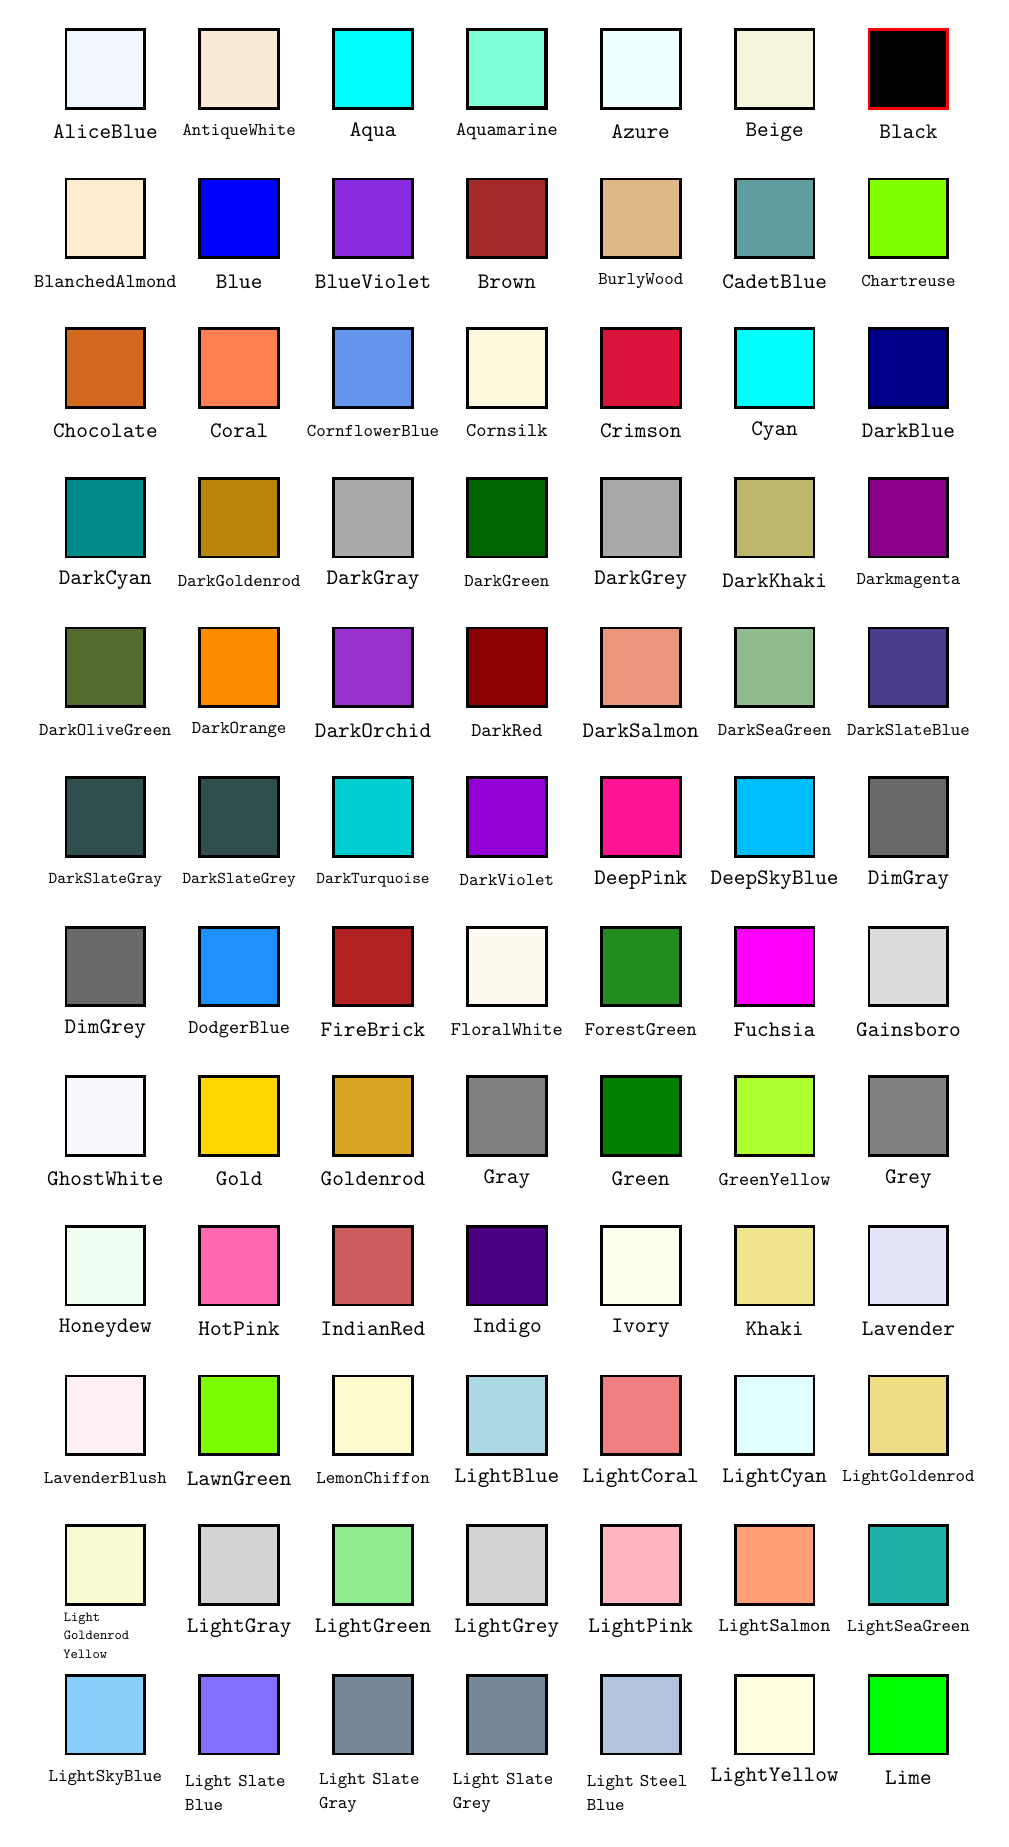
\begin{tikzpicture}

    \filldraw[draw=black,line width=1,fill=AliceBlue] (0,0) rectangle (1,1);

    \node[scale=0.8] at (0.5,-0.3) {\texttt{AliceBlue}};



    \begin{scope}[xshift=1.7cm]

      \filldraw[draw=black,line width=1,fill=AntiqueWhite]
      (0,0) rectangle (1,1);

      \node[scale=0.65] at (0.5,-0.3) {\texttt{AntiqueWhite}};

    \end{scope}



    \begin{scope}[xshift=3.4cm]

      \filldraw[draw=black,line width=1,fill=Aqua] (0,0) rectangle (1,1);

      \node[scale=0.8] at (0.5,-0.3) {\texttt{Aqua}};

    \end{scope}



    \begin{scope}[xshift=5.1cm]

      \filldraw[draw=black,line width=1.3,fill=Aquamarine]
      (0,0) rectangle (1,1);

      \node[scale=0.7] at (0.5,-0.3) {\texttt{Aquamarine}};

    \end{scope}



    \begin{scope}[xshift=6.8cm]

      \filldraw[draw=black,line width=1,fill=Azure] (0,0) rectangle (1,1);

      \node[scale=0.8] at (0.5,-0.3) {\texttt{Azure}};

    \end{scope}



    \begin{scope}[xshift=8.5cm]

      \filldraw[draw=black,line width=1,fill=Beige] (0,0) rectangle (1,1);

      \node[scale=0.8] at (0.5,-0.3) {\texttt{Beige}};

    \end{scope}



    \begin{scope}[xshift=10.2cm]

      \filldraw[draw=red,line width=1,fill=Black] (0,0) rectangle (1,1);

      \node[scale=0.8] at (0.5,-0.3) {\texttt{Black}};

    \end{scope}





    \begin{scope}[yshift=-1.9cm]

      \filldraw[draw=black,line width=1,fill=BlanchedAlmond]
      (0,0) rectangle (1,1);

      \node[scale=0.7] at (0.5,-0.3) {\texttt{BlanchedAlmond}};

    \end{scope}



    \begin{scope}[xshift=1.7cm,yshift=-1.9cm]

      \filldraw[draw=black,line width=1,fill=Blue] (0,0) rectangle (1,1);

      \node[scale=0.8] at (0.5,-0.3) {\texttt{Blue}};

    \end{scope}



    \begin{scope}[xshift=3.4cm,yshift=-1.9cm]

      \filldraw[draw=black,line width=1,fill=BlueViolet]
      (0,0) rectangle (1,1);

      \node[scale=0.8] at (0.5,-0.3) {\texttt{BlueViolet}};

    \end{scope}



    \begin{scope}[xshift=5.1cm,yshift=-1.9cm]

      \filldraw[draw=black,line width=1,fill=Brown] (0,0) rectangle (1,1);

      \node[scale=0.8] at (0.5,-0.3) {\texttt{Brown}};

    \end{scope}



    \begin{scope}[xshift=6.8cm,yshift=-1.9cm]

      \filldraw[draw=black,line width=1,fill=BurlyWood]
      (0,0) rectangle (1,1);

      \node[scale=0.65] at (0.5,-0.3) {\texttt{BurlyWood}};

    \end{scope}



    \begin{scope}[xshift=8.5cm,yshift=-1.9cm]

      \filldraw[draw=black,line width=1,fill=CadetBlue]
      (0,0) rectangle (1,1);

      \node[scale=0.8] at (0.5,-0.3) {\texttt{CadetBlue}};

    \end{scope}



    \begin{scope}[xshift=10.2cm,yshift=-1.9cm]

      \filldraw[draw=black,line width=1,fill=Chartreuse]
      (0,0) rectangle (1,1);

      \node[scale=0.65] at (0.5,-0.3) {\texttt{Chartreuse}};

    \end{scope}





    \begin{scope}[yshift=-3.8cm]

      \filldraw[draw=black,line width=1,fill=Chocolate]
      (0,0) rectangle (1,1);

      \node[scale=0.8] at (0.5,-0.3) {\texttt{Chocolate}};

    \end{scope}



    \begin{scope}[xshift=1.7cm,yshift=-3.8cm]

      \filldraw[draw=black,line width=1,fill=Coral] (0,0) rectangle (1,1);

      \node[scale=0.8] at (0.5,-0.3) {\texttt{Coral}};

    \end{scope}



    \begin{scope}[xshift=3.4cm,yshift=-3.8cm]

      \filldraw[draw=black,line width=1,fill=CornflowerBlue]
      (0,0) rectangle (1,1);

      \node[scale=0.65] at (0.5,-0.3) {\texttt{CornflowerBlue}};

    \end{scope}



    \begin{scope}[xshift=5.1cm,yshift=-3.8cm]

      \filldraw[draw=black,line width=1,fill=Cornsilk]
      (0,0) rectangle (1,1);

      \node[scale=0.7] at (0.5,-0.3) {\texttt{Cornsilk}};

    \end{scope}



    \begin{scope}[xshift=6.8cm,yshift=-3.8cm]

      \filldraw[draw=black,line width=1,fill=Crimson] (0,0) rectangle (1,1);

      \node[scale=0.8] at (0.5,-0.3) {\texttt{Crimson}};

    \end{scope}



    \begin{scope}[xshift=8.5cm,yshift=-3.8cm]

      \filldraw[draw=black,line width=1,fill=Cyan] (0,0) rectangle (1,1);

      \node[scale=0.8] at (0.5,-0.3) {\texttt{Cyan}};

    \end{scope}



    \begin{scope}[xshift=10.2cm,yshift=-3.8cm]

      \filldraw[draw=black,line width=1,fill=DarkBlue]
      (0,0) rectangle (1,1);

      \node[scale=0.8] at (0.5,-0.3) {\texttt{DarkBlue}};

    \end{scope}





    \begin{scope}[yshift=-5.7cm]

      \filldraw[draw=black,line width=1,fill=DarkCyan]
      (0,0) rectangle (1,1);

      \node[scale=0.8] at (0.5,-0.3) {\texttt{DarkCyan}};

    \end{scope}



    \begin{scope}[xshift=1.7cm,yshift=-5.7cm]

      \filldraw[draw=black,line width=1,fill=DarkGoldenrod]
      (0,0) rectangle (1,1);

      \node[scale=0.65] at (0.5,-0.3) {\texttt{DarkGoldenrod}};

    \end{scope}



    \begin{scope}[xshift=3.4cm,yshift=-5.7cm]

      \filldraw[draw=black,line width=1,fill=DarkGray]
      (0,0) rectangle (1,1);

      \node[scale=0.8] at (0.5,-0.3) {\texttt{DarkGray}};

    \end{scope}



    \begin{scope}[xshift=5.1cm,yshift=-5.7cm]

      \filldraw[draw=black,line width=1,fill=DarkGreen]
      (0,0) rectangle (1,1);

      \node[scale=0.65] at (0.5,-0.3) {\texttt{DarkGreen}};

    \end{scope}



    \begin{scope}[xshift=6.8cm,yshift=-5.7cm]

      \filldraw[draw=black,line width=1,fill=DarkGrey]
      (0,0) rectangle (1,1);

      \node[scale=0.8] at (0.5,-0.3) {\texttt{DarkGrey}};

    \end{scope}



    \begin{scope}[xshift=8.5cm,yshift=-5.7cm]

      \filldraw[draw=black,line width=1,fill=DarkKhaki]
      (0,0) rectangle (1,1);

      \node[scale=0.8] at (0.5,-0.3) {\texttt{DarkKhaki}};

    \end{scope}



    \begin{scope}[xshift=10.2cm,yshift=-5.7cm]

      \filldraw[draw=black,line width=1,fill=DarkMagenta]
      (0,0) rectangle (1,1);

      \node[scale=0.65] at (0.5,-0.3) {\texttt{Darkmagenta}};

    \end{scope}





    \begin{scope}[yshift=-7.6cm]

      \filldraw[draw=black,line width=1,fill=DarkOliveGreen]
      (0,0) rectangle (1,1);

      \node[scale=0.65] at (0.5,-0.3) {\texttt{DarkOliveGreen}};

    \end{scope}



    \begin{scope}[xshift=1.7cm,yshift=-7.6cm]

      \filldraw[draw=black,line width=1,fill=DarkOrange]
      (0,0) rectangle (1,1);

      \node[scale=0.65] at (0.5,-0.3) {\texttt{DarkOrange}};

    \end{scope}



    \begin{scope}[xshift=3.4cm,yshift=-7.6cm]

      \filldraw[draw=black,line width=1,fill=DarkOrchid]
      (0,0) rectangle (1,1);

      \node[scale=0.8] at (0.5,-0.3) {\texttt{DarkOrchid}};

    \end{scope}



    \begin{scope}[xshift=5.1cm,yshift=-7.6cm]

      \filldraw[draw=black,line width=1,fill=DarkRed] (0,0) rectangle (1,1);

      \node[scale=0.7] at (0.5,-0.3) {\texttt{DarkRed}};

    \end{scope}



    \begin{scope}[xshift=6.8cm,yshift=-7.6cm]

      \filldraw[draw=black,line width=1,fill=DarkSalmon]
      (0,0) rectangle (1,1);

      \node[scale=0.8] at (0.5,-0.3) {\texttt{DarkSalmon}};

    \end{scope}



    \begin{scope}[xshift=8.5cm,yshift=-7.6cm]

      \filldraw[draw=black,line width=1,fill=DarkSeaGreen]
      (0,0) rectangle (1,1);

      \node[scale=0.65] at (0.5,-0.3) {\texttt{DarkSeaGreen}};

    \end{scope}



    \begin{scope}[xshift=10.2cm,yshift=-7.6cm]

      \filldraw[draw=black,line width=1,fill=DarkSlateBlue]
      (0,0) rectangle (1,1);

      \node[scale=0.65] at (0.5,-0.3) {\texttt{DarkSlateBlue}};

    \end{scope}





    \begin{scope}[yshift=-9.5cm]

      \filldraw[draw=black,line width=1,fill=DarkSlateGray]
      (0,0) rectangle (1,1);

      \node[scale=0.6] at (0.5,-0.3) {\texttt{DarkSlateGray}};

    \end{scope}



    \begin{scope}[xshift=1.7cm,yshift=-9.5cm]

      \filldraw[draw=black,line width=1,fill=DarkSlateGrey]
      (0,0) rectangle (1,1);

      \node[scale=0.6] at (0.5,-0.3) {\texttt{DarkSlateGrey}};

    \end{scope}



    \begin{scope}[xshift=3.4cm,yshift=-9.5cm]

      \filldraw[draw=black,line width=1,fill=DarkTurquoise]
      (0,0) rectangle (1,1);

      \node[scale=0.6] at (0.5,-0.3) {\texttt{DarkTurquoise}};

    \end{scope}



    \begin{scope}[xshift=5.1cm,yshift=-9.5cm]

      \filldraw[draw=black,line width=1,fill=DarkViolet]
      (0,0) rectangle (1,1);

      \node[scale=0.65] at (0.5,-0.3) {\texttt{DarkViolet}};

    \end{scope}



    \begin{scope}[xshift=6.8cm,yshift=-9.5cm]

      \filldraw[draw=black,line width=1,fill=DeepPink]
      (0,0) rectangle (1,1);

      \node[scale=0.8] at (0.5,-0.3) {\texttt{DeepPink}};

    \end{scope}



    \begin{scope}[xshift=8.5cm,yshift=-9.5cm]

      \filldraw[draw=black,line width=1,fill=DeepSkyBlue]
      (0,0) rectangle (1,1);

      \node[scale=0.8] at (0.5,-0.3) {\texttt{DeepSkyBlue}};

    \end{scope}



    \begin{scope}[xshift=10.2cm,yshift=-9.5cm]

      \filldraw[draw=black,line width=1,fill=DimGray] (0,0) rectangle (1,1);

      \node[scale=0.8] at (0.5,-0.3) {\texttt{DimGray}};

    \end{scope}





    \begin{scope}[yshift=-11.4cm]

      \filldraw[draw=black,line width=1,fill=DimGrey] (0,0) rectangle (1,1);

      \node[scale=0.8] at (0.5,-0.3) {\texttt{DimGrey}};

    \end{scope}



    \begin{scope}[xshift=1.7cm,yshift=-11.4cm]

      \filldraw[draw=black,line width=1,fill=DodgerBlue]
      (0,0) rectangle (1,1);

      \node[scale=0.7] at (0.5,-0.3) {\texttt{DodgerBlue}};

    \end{scope}



    \begin{scope}[xshift=3.4cm,yshift=-11.4cm]

      \filldraw[draw=black,line width=1,fill=FireBrick]
      (0,0) rectangle (1,1);

      \node[scale=0.8] at (0.5,-0.3) {\texttt{FireBrick}};

    \end{scope}



    \begin{scope}[xshift=5.1cm,yshift=-11.4cm]

      \filldraw[draw=black,line width=1,fill=FloralWhite]
      (0,0) rectangle (1,1);

      \node[scale=0.7] at (0.5,-0.3) {\texttt{FloralWhite}};

    \end{scope}



    \begin{scope}[xshift=6.8cm,yshift=-11.4cm]

      \filldraw[draw=black,line width=1,fill=ForestGreen]
      (0,0) rectangle (1,1);

      \node[scale=0.7] at (0.5,-0.3) {\texttt{ForestGreen}};

    \end{scope}



    \begin{scope}[xshift=8.5cm,yshift=-11.4cm]

      \filldraw[draw=black,line width=1,fill=Fuchsia] (0,0) rectangle (1,1);

      \node[scale=0.8] at (0.5,-0.3) {\texttt{Fuchsia}};

    \end{scope}



    \begin{scope}[xshift=10.2cm,yshift=-11.4cm]

      \filldraw[draw=black,line width=1,fill=Gainsboro]
      (0,0) rectangle (1,1);

      \node[scale=0.8] at (0.5,-0.3) {\texttt{Gainsboro}};

    \end{scope}





    \begin{scope}[yshift=-13.3cm]

      \filldraw[draw=black,line width=1,fill=GhostWhite]
      (0,0) rectangle (1,1);

      \node[scale=0.8] at (0.5,-0.3) {\texttt{GhostWhite}};

    \end{scope}



    \begin{scope}[xshift=1.7cm,yshift=-13.3cm]

      \filldraw[draw=black,line width=1,fill=Gold] (0,0) rectangle (1,1);

      \node[scale=0.8] at (0.5,-0.3) {\texttt{Gold}};

    \end{scope}



    \begin{scope}[xshift=3.4cm,yshift=-13.3cm]

      \filldraw[draw=black,line width=1,fill=Goldenrod]
      (0,0) rectangle (1,1);

      \node[scale=0.8] at (0.5,-0.3) {\texttt{Goldenrod}};

    \end{scope}



    \begin{scope}[xshift=5.1cm,yshift=-13.3cm]

      \filldraw[draw=black,line width=1,fill=Gray] (0,0) rectangle (1,1);

      \node[scale=0.8] at (0.5,-0.3) {\texttt{Gray}};

    \end{scope}



    \begin{scope}[xshift=6.8cm,yshift=-13.3cm]

      \filldraw[draw=black,line width=1,fill=Green] (0,0) rectangle (1,1);

      \node[scale=0.8] at (0.5,-0.3) {\texttt{Green}};

    \end{scope}



    \begin{scope}[xshift=8.5cm,yshift=-13.3cm]

      \filldraw[draw=black,line width=1,fill=GreenYellow]
      (0,0) rectangle (1,1);

      \node[scale=0.7] at (0.5,-0.3) {\texttt{GreenYellow}};

    \end{scope}



    \begin{scope}[xshift=10.2cm,yshift=-13.3cm]

      \filldraw[draw=black,line width=1,fill=Grey] (0,0) rectangle (1,1);

      \node[scale=0.8] at (0.5,-0.3) {\texttt{Grey}};

    \end{scope}





    \begin{scope}[yshift=-15.2cm]

      \filldraw[draw=black,line width=1,fill=Honeydew]
      (0,0) rectangle (1,1);

      \node[scale=0.8] at (0.5,-0.3) {\texttt{Honeydew}};

    \end{scope}



    \begin{scope}[xshift=1.7cm,yshift=-15.2cm]

      \filldraw[draw=black,line width=1,fill=HotPink] (0,0) rectangle (1,1);

      \node[scale=0.8] at (0.5,-0.3) {\texttt{HotPink}};

    \end{scope}



    \begin{scope}[xshift=3.4cm,yshift=-15.2cm]

      \filldraw[draw=black,line width=1,fill=IndianRed]
      (0,0) rectangle (1,1);

      \node[scale=0.8] at (0.5,-0.3) {\texttt{IndianRed}};

    \end{scope}



    \begin{scope}[xshift=5.1cm,yshift=-15.2cm]

      \filldraw[draw=black,line width=1,fill=Indigo] (0,0) rectangle (1,1);

      \node[scale=0.8] at (0.5,-0.3) {\texttt{Indigo}};

    \end{scope}



    \begin{scope}[xshift=6.8cm,yshift=-15.2cm]

      \filldraw[draw=black,line width=1,fill=Ivory] (0,0) rectangle (1,1);

      \node[scale=0.8] at (0.5,-0.3) {\texttt{Ivory}};

    \end{scope}



    \begin{scope}[xshift=8.5cm,yshift=-15.2cm]

      \filldraw[draw=black,line width=1,fill=Khaki] (0,0) rectangle (1,1);

      \node[scale=0.8] at (0.5,-0.3) {\texttt{Khaki}};

    \end{scope}



    \begin{scope}[xshift=10.2cm,yshift=-15.2cm]

      \filldraw[draw=black,line width=1,fill=Lavender]
      (0,0) rectangle (1,1);

      \node[scale=0.8] at (0.5,-0.3) {\texttt{Lavender}};

    \end{scope}





    \begin{scope}[yshift=-17.1cm]

      \filldraw[draw=black,line width=1,fill=LavenderBlush]
      (0,0) rectangle (1,1);

      \node[scale=0.65] at (0.5,-0.3) {\texttt{LavenderBlush}};

    \end{scope}



    \begin{scope}[xshift=1.7cm,yshift=-17.1cm]

      \filldraw[draw=black,line width=1,fill=LawnGreen]
      (0,0) rectangle (1,1);

      \node[scale=0.8] at (0.5,-0.3) {\texttt{LawnGreen}};

    \end{scope}



    \begin{scope}[xshift=3.4cm,yshift=-17.1cm]

      \filldraw[draw=black,line width=1,fill=LemonChiffon]
      (0,0) rectangle (1,1);

      \node[scale=0.65] at (0.5,-0.3) {\texttt{LemonChiffon}};

    \end{scope}



    \begin{scope}[xshift=5.1cm,yshift=-17.1cm]

      \filldraw[draw=black,line width=1,fill=LightBlue]
      (0,0) rectangle (1,1);

      \node[scale=0.8] at (0.5,-0.3) {\texttt{LightBlue}};

    \end{scope}



    \begin{scope}[xshift=6.8cm,yshift=-17.1cm]

      \filldraw[draw=black,line width=1,fill=LightCoral]
      (0,0) rectangle (1,1);

      \node[scale=0.8] at (0.5,-0.3) {\texttt{LightCoral}};

    \end{scope}



    \begin{scope}[xshift=8.5cm,yshift=-17.1cm]

      \filldraw[draw=black,line width=1,fill=LightCyan]
      (0,0) rectangle (1,1);

      \node[scale=0.8] at (0.5,-0.3) {\texttt{LightCyan}};

    \end{scope}



    \begin{scope}[xshift=10.2cm,yshift=-17.1cm]

      \filldraw[draw=black,line width=1,fill=LightGoldenrod]
      (0,0) rectangle (1,1);

      \node[scale=0.65] at (0.5,-0.3) {\texttt{LightGoldenrod}};

    \end{scope}





    \begin{scope}[yshift=-19cm]

      \filldraw[draw=black,line width=1,fill=LightGoldenrodYellow]
      (0,0) rectangle (1,1);

      \node[scale=0.5,text width=6em] at (0.5,-0.4)
      {\texttt{Light Goldenrod Yellow}};

    \end{scope}



    \begin{scope}[xshift=1.7cm,yshift=-19cm]

      \filldraw[draw=black,line width=1,fill=LightGray]
      (0,0) rectangle (1,1);

      \node[scale=0.8] at (0.5,-0.3) {\texttt{LightGray}};

    \end{scope}



    \begin{scope}[xshift=3.4cm,yshift=-19cm]

      \filldraw[draw=black,line width=1,fill=LightGreen]
      (0,0) rectangle (1,1);

      \node[scale=0.8] at (0.5,-0.3) {\texttt{LightGreen}};

    \end{scope}



    \begin{scope}[xshift=5.1cm,yshift=-19cm]

      \filldraw[draw=black,line width=1,fill=LightGrey]
      (0,0) rectangle (1,1);

      \node[scale=0.8] at (0.5,-0.3) {\texttt{LightGrey}};

    \end{scope}



    \begin{scope}[xshift=6.8cm,yshift=-19cm]

      \filldraw[draw=black,line width=1,fill=LightPink]
      (0,0) rectangle (1,1);

      \node[scale=0.8] at (0.5,-0.3) {\texttt{LightPink}};

    \end{scope}



    \begin{scope}[xshift=8.5cm,yshift=-19cm]

      \filldraw[draw=black,line width=1,fill=LightSalmon]
      (0,0) rectangle (1,1);

      \node[scale=0.7] at (0.5,-0.3) {\texttt{LightSalmon}};

    \end{scope}



    \begin{scope}[xshift=10.2cm,yshift=-19cm]

      \filldraw[draw=black,line width=1,fill=LightSeaGreen]
      (0,0) rectangle (1,1);

      \node[scale=0.65] at (0.5,-0.3) {\texttt{LightSeaGreen}};

    \end{scope}





    \begin{scope}[yshift=-20.9cm]

      \filldraw[draw=black,line width=1,fill=LightSkyBlue]
      (0,0) rectangle (1,1);

      \node[scale=0.65] at (0.5,-0.3) {\texttt{LightSkyBlue}};

    \end{scope}



    \begin{scope}[xshift=1.7cm,yshift=-20.9cm]

      \filldraw[draw=black,line width=1,fill=LightSlateBlue]
      (0,0) rectangle (1,1);

      \node[scale=0.65,text width=6em] at (0.5,-0.5)
      {\texttt{Light Slate Blue}};

    \end{scope}



    \begin{scope}[xshift=3.4cm,yshift=-20.9cm]

      \filldraw[draw=black,line width=1,fill=LightSlateGray]
      (0,0) rectangle (1,1);

      \node[scale=0.65,text width=6em] at (0.5,-0.5)
      {\texttt{Light Slate Gray}};

    \end{scope}



    \begin{scope}[xshift=5.1cm,yshift=-20.9cm]

      \filldraw[draw=black,line width=1,fill=LightSlateGrey]
      (0,0) rectangle (1,1);

      \node[scale=0.65,text width=6em] at (0.5,-0.5)
      {\texttt{Light Slate Grey}};

    \end{scope}



    \begin{scope}[xshift=6.8cm,yshift=-20.9cm]

      \filldraw[draw=black,line width=1,fill=LightSteelBlue]
      (0,0) rectangle (1,1);

      \node[scale=0.65,text width=6em] at (0.5,-0.5)
      {\texttt{Light Steel Blue}};

    \end{scope}



    \begin{scope}[xshift=8.5cm,yshift=-20.9cm]

      \filldraw[draw=black,line width=1,fill=LightYellow]
      (0,0) rectangle (1,1);

      \node[scale=0.8] at (0.5,-0.3) {\texttt{LightYellow}};

    \end{scope}



    \begin{scope}[xshift=10.2cm,yshift=-20.9cm]

      \filldraw[draw=black,line width=1,fill=Lime] (0,0) rectangle (1,1);

      \node[scale=0.8] at (0.5,-0.3) {\texttt{Lime}};

    \end{scope}

  \end{tikzpicture}

  \caption{Kolor grupy \texttt{svgnames} z~paczki
    \href{https://ctan.org/pkg/xcolor}{\texttt{xcolor}}}


  \label{fig:svgnames-colors-01}

\end{figure}
% ##################





% ##################
\begin{figure}

  \centering


  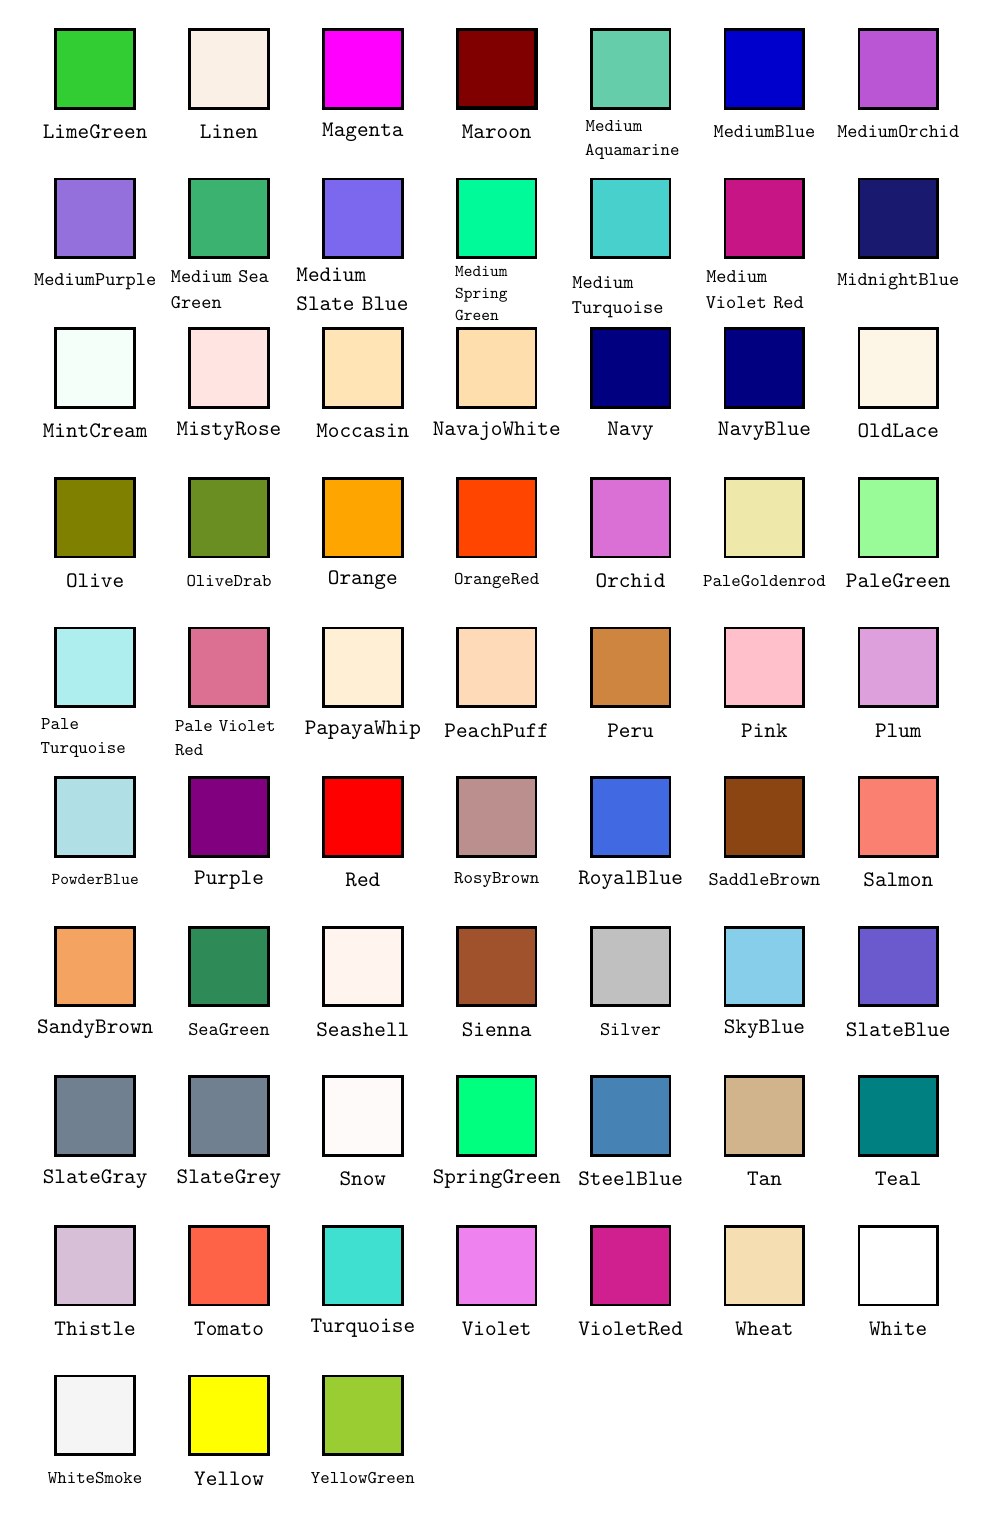
\begin{tikzpicture}

    \filldraw[draw=black,line width=1,fill=LimeGreen] (0,0) rectangle (1,1);

    \node[scale=0.8] at (0.5,-0.3) {\texttt{LimeGreen}};



    \begin{scope}[xshift=1.7cm]

      \filldraw[draw=black,line width=1,fill=Linen] (0,0) rectangle (1,1);

      \node[scale=0.8] at (0.5,-0.3) {\texttt{Linen}};

    \end{scope}



    \begin{scope}[xshift=3.4cm]

      \filldraw[draw=black,line width=1,fill=Magenta] (0,0) rectangle (1,1);

      \node[scale=0.8] at (0.5,-0.3) {\texttt{Magenta}};

    \end{scope}



    \begin{scope}[xshift=5.1cm]

      \filldraw[draw=black,line width=1.3,fill=Maroon]
      (0,0) rectangle (1,1);

      \node[scale=0.8] at (0.5,-0.3) {\texttt{Maroon}};

    \end{scope}



    \begin{scope}[xshift=6.8cm]

      \filldraw[draw=black,line width=1,fill=MediumAquamarine]
      (0,0) rectangle (1,1);

      \node[scale=0.65,text width=5em] at (0.5,-0.4)
      {\texttt{Medium Aquamarine}};

    \end{scope}



    \begin{scope}[xshift=8.5cm]

      \filldraw[draw=black,line width=1,fill=MediumBlue]
      (0,0) rectangle (1,1);

      \node[scale=0.7] at (0.5,-0.3) {\texttt{MediumBlue}};

    \end{scope}



    \begin{scope}[xshift=10.2cm]

      \filldraw[draw=black,line width=1,fill=MediumOrchid]
      (0,0) rectangle (1,1);

      \node[scale=0.7] at (0.5,-0.3) {\texttt{MediumOrchid}};

    \end{scope}





    \begin{scope}[yshift=-1.9cm]

      \filldraw[draw=black,line width=1,fill=MediumPurple]
      (0,0) rectangle (1,1);

      \node[scale=0.7] at (0.5,-0.3) {\texttt{MediumPurple}};

    \end{scope}



    \begin{scope}[xshift=1.7cm,yshift=-1.9cm]

      \filldraw[draw=black,line width=1,fill=MediumSeaGreen]
      (0,0) rectangle (1,1);

      \node[scale=0.7,text width=6em] at (0.5,-0.4)
      {\texttt{Medium Sea Green}};

    \end{scope}



    \begin{scope}[xshift=3.4cm,yshift=-1.9cm]

      \filldraw[draw=black,line width=1,fill=MediumSlateBlue]
      (0,0) rectangle (1,1);

      \node[scale=0.8,text width=6em] at (0.5,-0.4)
      {\texttt{Medium Slate Blue}};

    \end{scope}



    \begin{scope}[xshift=5.1cm,yshift=-1.9cm]

      \filldraw[draw=black,line width=1,fill=MediumSpringGreen]
      (0,0) rectangle (1,1);

      \node[scale=0.6,text width=5em] at (0.5,-0.45)
      {\texttt{Medium Spring Green}};

    \end{scope}



    \begin{scope}[xshift=6.8cm,yshift=-1.9cm]

      \filldraw[draw=black,line width=1,fill=MediumTurquoise]
      (0,0) rectangle (1,1);

      \node[scale=0.7,text width=6em] at (0.5,-0.5)
      {\texttt{Medium Turquoise}};

    \end{scope}



    \begin{scope}[xshift=8.5cm,yshift=-1.9cm]

      \filldraw[draw=black,line width=1,fill=MediumVioletRed]
      (0,0) rectangle (1,1);

      \node[scale=0.7,text width=6em] at (0.5,-0.4)
      {\texttt{Medium Violet Red}};

    \end{scope}



    \begin{scope}[xshift=10.2cm,yshift=-1.9cm]

      \filldraw[draw=black,line width=1,fill=MidnightBlue]
      (0,0) rectangle (1,1);

      \node[scale=0.7] at (0.5,-0.3) {\texttt{MidnightBlue}};

    \end{scope}





    \begin{scope}[yshift=-3.8cm]

      \filldraw[draw=black,line width=1,fill=MintCream]
      (0,0) rectangle (1,1);

      \node[scale=0.8] at (0.5,-0.3) {\texttt{MintCream}};

    \end{scope}



    \begin{scope}[xshift=1.7cm,yshift=-3.8cm]

      \filldraw[draw=black,line width=1,fill=MistyRose]
      (0,0) rectangle (1,1);

      \node[scale=0.8] at (0.5,-0.3) {\texttt{MistyRose}};

    \end{scope}



    \begin{scope}[xshift=3.4cm,yshift=-3.8cm]

      \filldraw[draw=black,line width=1,fill=Moccasin]
      (0,0) rectangle (1,1);

      \node[scale=0.8] at (0.5,-0.3) {\texttt{Moccasin}};

    \end{scope}



    \begin{scope}[xshift=5.1cm,yshift=-3.8cm]

      \filldraw[draw=black,line width=1,fill=NavajoWhite]
      (0,0) rectangle (1,1);

      \node[scale=0.8] at (0.5,-0.3) {\texttt{NavajoWhite}};

    \end{scope}



    \begin{scope}[xshift=6.8cm,yshift=-3.8cm]

      \filldraw[draw=black,line width=1,fill=Navy] (0,0) rectangle (1,1);

      \node[scale=0.8] at (0.5,-0.3) {\texttt{Navy}};

    \end{scope}



    \begin{scope}[xshift=8.5cm,yshift=-3.8cm]

      \filldraw[draw=black,line width=1,fill=NavyBlue]
      (0,0) rectangle (1,1);

      \node[scale=0.8] at (0.5,-0.3) {\texttt{NavyBlue}};

    \end{scope}



    \begin{scope}[xshift=10.2cm,yshift=-3.8cm]

      \filldraw[draw=black,line width=1,fill=OldLace] (0,0) rectangle (1,1);

      \node[scale=0.8] at (0.5,-0.3) {\texttt{OldLace}};

    \end{scope}





    \begin{scope}[yshift=-5.7cm]

      \filldraw[draw=black,line width=1,fill=Olive] (0,0) rectangle (1,1);

      \node[scale=0.8] at (0.5,-0.3) {\texttt{Olive}};

    \end{scope}



    \begin{scope}[xshift=1.7cm,yshift=-5.7cm]

      \filldraw[draw=black,line width=1,fill=OliveDrab]
      (0,0) rectangle (1,1);

      \node[scale=0.65] at (0.5,-0.3) {\texttt{OliveDrab}};

    \end{scope}



    \begin{scope}[xshift=3.4cm,yshift=-5.7cm]

      \filldraw[draw=black,line width=1,fill=Orange] (0,0) rectangle (1,1);

      \node[scale=0.8] at (0.5,-0.3) {\texttt{Orange}};

    \end{scope}



    \begin{scope}[xshift=5.1cm,yshift=-5.7cm]

      \filldraw[draw=black,line width=1,fill=OrangeRed]
      (0,0) rectangle (1,1);

      \node[scale=0.65] at (0.5,-0.3) {\texttt{OrangeRed}};

    \end{scope}



    \begin{scope}[xshift=6.8cm,yshift=-5.7cm]

      \filldraw[draw=black,line width=1,fill=Orchid]
      (0,0) rectangle (1,1);

      \node[scale=0.8] at (0.5,-0.3) {\texttt{Orchid}};

    \end{scope}



    \begin{scope}[xshift=8.5cm,yshift=-5.7cm]

      \filldraw[draw=black,line width=1,fill=PaleGoldenrod]
      (0,0) rectangle (1,1);

      \node[scale=0.65] at (0.5,-0.3) {\texttt{PaleGoldenrod}};

    \end{scope}



    \begin{scope}[xshift=10.2cm,yshift=-5.7cm]

      \filldraw[draw=black,line width=1,fill=PaleGreen]
      (0,0) rectangle (1,1);

      \node[scale=0.8] at (0.5,-0.3) {\texttt{PaleGreen}};

    \end{scope}





    \begin{scope}[yshift=-7.6cm]

      \filldraw[draw=black,line width=1,fill=PaleTurquoise]
      (0,0) rectangle (1,1);

      \node[scale=0.65,text width=6em] at (0.5,-0.4)
      {\texttt{Pale Turquoise}};

    \end{scope}



    \begin{scope}[xshift=1.7cm,yshift=-7.6cm]

      \filldraw[draw=black,line width=1,fill=PaleVioletRed]
      (0,0) rectangle (1,1);

      \node[scale=0.65,text width=6em] at (0.5,-0.4)
      {\texttt{Pale Violet Red}};

    \end{scope}



    \begin{scope}[xshift=3.4cm,yshift=-7.6cm]

      \filldraw[draw=black,line width=1,fill=PapayaWhip]
      (0,0) rectangle (1,1);

      \node[scale=0.8] at (0.5,-0.3) {\texttt{PapayaWhip}};

    \end{scope}



    \begin{scope}[xshift=5.1cm,yshift=-7.6cm]

      \filldraw[draw=black,line width=1,fill=PeachPuff]
      (0,0) rectangle (1,1);

      \node[scale=0.8] at (0.5,-0.3) {\texttt{PeachPuff}};

    \end{scope}



    \begin{scope}[xshift=6.8cm,yshift=-7.6cm]

      \filldraw[draw=black,line width=1,fill=Peru] (0,0) rectangle (1,1);

      \node[scale=0.8] at (0.5,-0.3) {\texttt{Peru}};

    \end{scope}



    \begin{scope}[xshift=8.5cm,yshift=-7.6cm]

      \filldraw[draw=black,line width=1,fill=Pink] (0,0) rectangle (1,1);

      \node[scale=0.8] at (0.5,-0.3) {\texttt{Pink}};

    \end{scope}



    \begin{scope}[xshift=10.2cm,yshift=-7.6cm]

      \filldraw[draw=black,line width=1,fill=Plum] (0,0) rectangle (1,1);

      \node[scale=0.8] at (0.5,-0.3) {\texttt{Plum}};

    \end{scope}





    \begin{scope}[yshift=-9.5cm]

      \filldraw[draw=black,line width=1,fill=PowderBlue]
      (0,0) rectangle (1,1);

      \node[scale=0.6] at (0.5,-0.3) {\texttt{PowderBlue}};

    \end{scope}



    \begin{scope}[xshift=1.7cm,yshift=-9.5cm]

      \filldraw[draw=black,line width=1,fill=Purple] (0,0) rectangle (1,1);

      \node[scale=0.8] at (0.5,-0.3) {\texttt{Purple}};

    \end{scope}



    \begin{scope}[xshift=3.4cm,yshift=-9.5cm]

      \filldraw[draw=black,line width=1,fill=Red] (0,0) rectangle (1,1);

      \node[scale=0.8] at (0.5,-0.3) {\texttt{Red}};

    \end{scope}



    \begin{scope}[xshift=5.1cm,yshift=-9.5cm]

      \filldraw[draw=black,line width=1,fill=RosyBrown]
      (0,0) rectangle (1,1);

      \node[scale=0.65] at (0.5,-0.3) {\texttt{RosyBrown}};

    \end{scope}



    \begin{scope}[xshift=6.8cm,yshift=-9.5cm]

      \filldraw[draw=black,line width=1,fill=RoyalBlue]
      (0,0) rectangle (1,1);

      \node[scale=0.8] at (0.5,-0.3) {\texttt{RoyalBlue}};

    \end{scope}



    \begin{scope}[xshift=8.5cm,yshift=-9.5cm]

      \filldraw[draw=black,line width=1,fill=SaddleBrown]
      (0,0) rectangle (1,1);

      \node[scale=0.7] at (0.5,-0.3) {\texttt{SaddleBrown}};

    \end{scope}



    \begin{scope}[xshift=10.2cm,yshift=-9.5cm]

      \filldraw[draw=black,line width=1,fill=Salmon] (0,0) rectangle (1,1);

      \node[scale=0.8] at (0.5,-0.3) {\texttt{Salmon}};

    \end{scope}





    \begin{scope}[yshift=-11.4cm]

      \filldraw[draw=black,line width=1,fill=SandyBrown]
      (0,0) rectangle (1,1);

      \node[scale=0.8] at (0.5,-0.3) {\texttt{SandyBrown}};

    \end{scope}



    \begin{scope}[xshift=1.7cm,yshift=-11.4cm]

      \filldraw[draw=black,line width=1,fill=SeaGreen]
      (0,0) rectangle (1,1);

      \node[scale=0.7] at (0.5,-0.3) {\texttt{SeaGreen}};

    \end{scope}



    \begin{scope}[xshift=3.4cm,yshift=-11.4cm]

      \filldraw[draw=black,line width=1,fill=Seashell]
      (0,0) rectangle (1,1);

      \node[scale=0.8] at (0.5,-0.3) {\texttt{Seashell}};

    \end{scope}



    \begin{scope}[xshift=5.1cm,yshift=-11.4cm]

      \filldraw[draw=black,line width=1,fill=Sienna] (0,0) rectangle (1,1);

      \node[scale=0.8] at (0.5,-0.3) {\texttt{Sienna}};

    \end{scope}



    \begin{scope}[xshift=6.8cm,yshift=-11.4cm]

      \filldraw[draw=black,line width=1,fill=Silver] (0,0) rectangle (1,1);

      \node[scale=0.7] at (0.5,-0.3) {\texttt{Silver}};

    \end{scope}



    \begin{scope}[xshift=8.5cm,yshift=-11.4cm]

      \filldraw[draw=black,line width=1,fill=SkyBlue] (0,0) rectangle (1,1);

      \node[scale=0.8] at (0.5,-0.3) {\texttt{SkyBlue}};

    \end{scope}



    \begin{scope}[xshift=10.2cm,yshift=-11.4cm]

      \filldraw[draw=black,line width=1,fill=SlateBlue]
      (0,0) rectangle (1,1);

      \node[scale=0.8] at (0.5,-0.3) {\texttt{SlateBlue}};

    \end{scope}





    \begin{scope}[yshift=-13.3cm]

      \filldraw[draw=black,line width=1,fill=SlateGray]
      (0,0) rectangle (1,1);

      \node[scale=0.8] at (0.5,-0.3) {\texttt{SlateGray}};

    \end{scope}



    \begin{scope}[xshift=1.7cm,yshift=-13.3cm]

      \filldraw[draw=black,line width=1,fill=SlateGrey]
      (0,0) rectangle (1,1);

      \node[scale=0.8] at (0.5,-0.3) {\texttt{SlateGrey}};

    \end{scope}



    \begin{scope}[xshift=3.4cm,yshift=-13.3cm]

      \filldraw[draw=black,line width=1,fill=Snow] (0,0) rectangle (1,1);

      \node[scale=0.8] at (0.5,-0.3) {\texttt{Snow}};

    \end{scope}



    \begin{scope}[xshift=5.1cm,yshift=-13.3cm]

      \filldraw[draw=black,line width=1,fill=SpringGreen]
      (0,0) rectangle (1,1);

      \node[scale=0.8] at (0.5,-0.3) {\texttt{SpringGreen}};

    \end{scope}



    \begin{scope}[xshift=6.8cm,yshift=-13.3cm]

      \filldraw[draw=black,line width=1,fill=SteelBlue]
      (0,0) rectangle (1,1);

      \node[scale=0.8] at (0.5,-0.3) {\texttt{SteelBlue}};

    \end{scope}



    \begin{scope}[xshift=8.5cm,yshift=-13.3cm]

      \filldraw[draw=black,line width=1,fill=Tan] (0,0) rectangle (1,1);

      \node[scale=0.8] at (0.5,-0.3) {\texttt{Tan}};

    \end{scope}



    \begin{scope}[xshift=10.2cm,yshift=-13.3cm]

      \filldraw[draw=black,line width=1,fill=Teal] (0,0) rectangle (1,1);

      \node[scale=0.8] at (0.5,-0.3) {\texttt{Teal}};

    \end{scope}





    \begin{scope}[yshift=-15.2cm]

      \filldraw[draw=black,line width=1,fill=Thistle] (0,0) rectangle (1,1);

      \node[scale=0.8] at (0.5,-0.3) {\texttt{Thistle}};

    \end{scope}



    \begin{scope}[xshift=1.7cm,yshift=-15.2cm]

      \filldraw[draw=black,line width=1,fill=Tomato] (0,0) rectangle (1,1);

      \node[scale=0.8] at (0.5,-0.3) {\texttt{Tomato}};

    \end{scope}



    \begin{scope}[xshift=3.4cm,yshift=-15.2cm]

      \filldraw[draw=black,line width=1,fill=Turquoise]
      (0,0) rectangle (1,1);

      \node[scale=0.8] at (0.5,-0.3) {\texttt{Turquoise}};

    \end{scope}



    \begin{scope}[xshift=5.1cm,yshift=-15.2cm]

      \filldraw[draw=black,line width=1,fill=Violet] (0,0) rectangle (1,1);

      \node[scale=0.8] at (0.5,-0.3) {\texttt{Violet}};

    \end{scope}



    \begin{scope}[xshift=6.8cm,yshift=-15.2cm]

      \filldraw[draw=black,line width=1,fill=VioletRed]
      (0,0) rectangle (1,1);

      \node[scale=0.8] at (0.5,-0.3) {\texttt{VioletRed}};

    \end{scope}



    \begin{scope}[xshift=8.5cm,yshift=-15.2cm]

      \filldraw[draw=black,line width=1,fill=Wheat] (0,0) rectangle (1,1);

      \node[scale=0.8] at (0.5,-0.3) {\texttt{Wheat}};

    \end{scope}



    \begin{scope}[xshift=10.2cm,yshift=-15.2cm]

      \filldraw[draw=black,line width=1,fill=White] (0,0) rectangle (1,1);

      \node[scale=0.8] at (0.5,-0.3) {\texttt{White}};

    \end{scope}





    \begin{scope}[yshift=-17.1cm]

      \filldraw[draw=black,line width=1,fill=WhiteSmoke]
      (0,0) rectangle (1,1);

      \node[scale=0.65] at (0.5,-0.3) {\texttt{WhiteSmoke}};

    \end{scope}



    \begin{scope}[xshift=1.7cm,yshift=-17.1cm]

      \filldraw[draw=black,line width=1,fill=Yellow] (0,0) rectangle (1,1);

      \node[scale=0.8] at (0.5,-0.3) {\texttt{Yellow}};

    \end{scope}



    \begin{scope}[xshift=3.4cm,yshift=-17.1cm]

      \filldraw[draw=black,line width=1,fill=YellowGreen]
      (0,0) rectangle (1,1);

      \node[scale=0.65] at (0.5,-0.3) {\texttt{YellowGreen}};

    \end{scope}

  \end{tikzpicture}

  \caption{Kolor grupy \texttt{svgnames} z~paczki
    \href{https://ctan.org/pkg/xcolor}{\texttt{xcolor}}}


  \label{fig:svgnames-colors-01}

\end{figure}
% ##################
















% ####################################################################
% ####################################################################
% Bibliography

% \printbibliography





% ############################
% End of the document

\end{document}
